\chapter{Реализация Allure Framework} 
\label{chapter3}

\section{Разработка Allure Framework}

В этой главе можно узнать про процесс разработки фремворка Allure.

\subsection{Первые шаги}

После исследования была поставлена задача написать первый прототип. Решено было писать прототип для связки JUnit + Maven, так как именно эти технологии в основном использовались в компании Яндекс. 

Проект был поделен на два модуля: адаптер для JUnit, который собирал данные о ходе теста, и плагин для Maven, который генерировал по этим данным отчет. Адаптер представлял из себя две JUnit рулы, одна собирала информацию о тесте, другая о тест суите. Для того, чтобы начать собирать информацию о тесте, необходимо было добавить в код теста:

\begin{lstlisting}
@ClassRule
public static TestSuiteReportRule testSuite = new TestSuiteReportRule();

@Rule
public TestCaseReportRule testCase = new TestCaseReportRule(testSuite, this);
\end{lstlisting}


Генерация отчета происходила с помощью шаблонизатора freemarker. 

Реализация шагов и аттачментов в прототипе была достаточно сложной --- использовалась библиотека cglib, которая накладывала много ограничений на методы шагов и методы сохранения аттачментов.

Прототип был написан в сентябре 2013 года, начал внедряться в некоторые новые тестовые проекты в компании Яндекс.

\subsection{Подключение прототипа к существующим проектам}

Прототип уже использовался в некоторых новых тестовых проектах, но подключение к существующим тестам все еще было большой проблемой. Ведь для того, чтобы добавить в каждый тест (а в небольших тестовых проектах их около 500) две строчки надо было затратить существенное количество времени. 

Тогда было решено воспользоваться инструментацией кода. Инструментация --- это некоторое изменение байт-кода программы. Для решения этой задачи выбор пал на фреймворк ASM OW2. Автором работы был написан Maven плагин, который после компиляции проекта во все тесты инжектировал Allure рулы. Тем самым появилась возможность генерировать отчет для больших уже написанных проектов.

\subsection{PyTest}

Сразу после окончания разработки прототипа поступил запрос от команды тестировщиков, которые писали тесты на Python с использованием PyTest. Дело в том, что для языка программирования python, а в частности фремворка PyTest не было возможности построить отчет, кроме стандартного surefire. Но возможностей surefire тестировщикам не хватало, и большую часть времени тестирования занимал анализ логов тестов.

С этого момента начался следующий цикл разработки Allure. Автор данной работы начал пытаться адаптировать текущий прототип под Python. Произошли существенные изменения в модели --- стало понятно, что большинство логики JUnit-адаптера будет дублироваться в PyTest-адаптере.
Было решено разделить модель на два уровня. Первый уровень должен содержать только несентезируемые, чистые данные, а второй --- содержать данные в удобном для отображения формате. Появился новый модуль, получивший название Report Generator (генератор отчета). 
В данный модуль была вынесена общая логика из JUnit и PyTest адаптеров.

Следующим этапом было написание Jenkins плагина. Дело в том, что тесты на Python не использут Maven в своем жизненном цикле. В конкретно нашем случае они запускались с использованием Jenkins. Чтобы не устанавливать Maven на виртуальные машины, на которых запускались тесты, было решено написать плагин для Jenkins. 

\subsection{AspectJ}

Несмотря на то, что фремворк уже начали использовать в некоторых проектах, большая часть проектов отказывалась подлючать Allure из-за сложностей с шагами. Дело в том, что шаги определялись очень сложным образом, и перевести существующие библиотеки шагов на предлагаемый способ подключения не предоставлялось возможным. Тогда было решено использовать фремворк AspectJ для сбора информации о пройденых шагах. Данный фремворк позволяет встроить некоторый код в байт-код загружаемого ClassLoader'ом класса. Притом, не надо думать об устройстве и структуре байт кода, достаточно просто описать  точки входа (pointcuts) и аспекты (aspects): 

\begin{lstlisting}
@Pointcut("@annotation(ru.yandex.qatools.allure.annotations.Step)")
public void withStepAnnotation() {
    //pointcut body, should be empty
}

@Pointcut("execution(* *(..))")
public void anyMethod() {
    //pointcut body, should be empty
}

@Before("anyMethod() && withStepAnnotation()")
public void stepStart(JoinPoint joinPoint) {
    ...
}

@AfterThrowing(pointcut = "anyMethod() && withStepAnnotation()", throwing = "e")
public void stepFailed(JoinPoint joinPoint, Throwable e) {
    ...
}

@AfterReturning(pointcut = "anyMethod() && withStepAnnotation()", returning = "result")
public void stepStop(JoinPoint joinPoint, Object result) {
    ...
}
\end{lstlisting}


В итоге для добавления шага надо проаннатировать метод аннотацией @Step. 

\newpage
\subsection{Примеры работы фреймворка Allure для JUnit тестов}

Уже на данном этапе одно из основных достоинств разработаного автором фреймворка является прозрачная интеграция с существующими тестовыми системами. Рассмотрим простейший JUnit тест:
 
\begin{lstlisting}
public class SimpleTest {

    @Test
    public void simpleTest() throws Exception {
        assertThat(4, is(2 + 2));
    }
    
    public int sum(int a, int b) {
		return a + b;
	}    
    
    public void check(int a, int b, int c) {
    	assertThat(c, is(a + b));	
    }
}
\end{lstlisting}

Для данного теста уже можно построить отчет. Достаточно воспользоваться одним из инструментов для генерации отчета.

Чтобы отобразить информацию о тестовом сценарии достаточно проаннотировать соответствующие методы аннотацией @Step.

\begin{lstlisting}
public class SimpleTest {

    @Test
    public void simpleTest() throws Exception {
        int c = sum(2, 2);
        check(2, 2, c);
    }
    
    @Step("Считаем сумму '{0}' и '{1}'")
    public int sum(int a, int b) {
		return a + b;
	}    
    
    @Step("Проверяем, что сумма '{0}' и '{1}' равна '{c}'")
    public void check(int a, int b, int c) {
    	assertThat(c, is(a + b));	
    }
}
\end{lstlisting}

Так же просто мы может добавлять к тесту аттачменты, указывать параметры, группировать тесты по требованиям и историям, и так далее.

\subsection{TestNG}

В качестве эксперимента автором работы был написан адаптер для TestNG. то второй поддерживаемый тестовый фреймворк для Java, написание которого показало необходимость в новом слое абстракции, API для языка программирования. После этого код самих адаптеров сильно упростился. Также пропала необходимость использовать тестовые фремворки для проверок. Отчет можно построить по результатам выполнения любого кода, достаточно лишь определить, что является тестом, а что проверкой.

\subsection{Report Face}

Как только фреймворк начал набирать популярность, стало появляться все больше требований к самому отчету. Было решено заменить freemarker на AngularJS и сделать отчет в виде One-Page-Application. 

\subsection{Report Face 2.0}

Автор данной работы на момент написания работы не является профессиональным Java Script разработчком, из-за чего возникало множество проблем в отчете. Поэтому к разработке присоеденился Борис Сердюк, который полностью переработал структуру отчета, и воплотил в жизнь все задумки.

\subsection{Остальные фреймворки}

По мере развития Allure появлялась поддержка новых фреймворков и способов построения отчета:

\begin{itemize}
\item TestNG --- адаптер для данного языка был написан автором данной работы.
\item RSpec -- адаптер написан Ильей Садыковым.
\item PHPUnit --- адаптер написан Иваном Крутовым.
\item ScalaTest --- адаптер написан Иваном Крутовым.
\item Karma --- адаптер написал Борис Сердюк, данный адаптер позволяет строить отчет для тестов, спользующих Karma, например, Jasmine-тестов.
\item TeamCity Plugin --- плагин написан Иваном Крутовым. Добавляет возможность строить отчет в TeanCity.
\item Command Line Interface ---написан Иваном Крутовым совместно с автором данной работы. Позволяет строить отчет используя коммандную строку.
\end{itemize}

\subsection{Report Generation API}

На данный момент в связи с появлением большого количества инструментов, позволяющих генерировать отчет, разрабатывается библиотека, генерирующая отчет. В ней будут описаны все методы, которые нужны для построения отчета. 

\section{Общая схема работы} 

После разработки прототипа было еще много изменений в структуре проекта. Весь код переписывался, четыре раза. На данный момент автор работает над версией 1.4. В данном разделе описывается текущее состояние фреймворка.

Общая схема работы Allure показана на рисунке \ref{fig:allure}. Рассмотрим подробнее назначение отдельных частей.

\begin{figure}[htb]
\centering
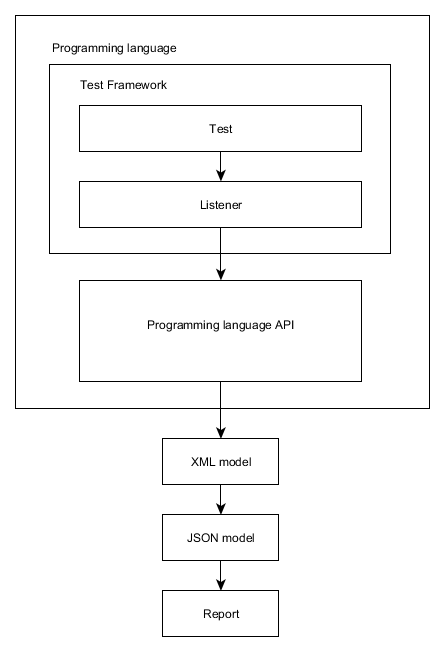
\includegraphics[height=160mm]{structure.png}
\caption{Общая схема фремворка Allure}
\label{fig:allure}
\end{figure}

\subsection{Listener}

Для большинства тестовых фремворков xUnit есть возможность подключить листенер для сбора информации о ходе тестов. Мало того, подключение листенера, как правило, вынесено на уровень конфигурации запуска, что полностью удавлетворяет требованиям работы. Для адаптации тестового фремворка достаточно реализовать тест листенер используя соответсвующее API языка программирования.

Однако стоит заметить, что не всю необходимую информацию о ходе теста можно собрать используя листенер, так как он оперирует терминологией xUnit. Сбор остальной информации о тестах, например информацию о пройденных шагах и сделанных аттачментах, будет реализован на уровне API языка программирования.

\subsection{Programming language API}

API для языка программирования представляет из себя набор обработчиков событий и сами события, используя которые можно полностью описать жизненный цикл теста. Программный инетрфейс содержит в себе следующие события:

\begin{itemize}
\item начало/конец тестового запуска;
\item начало/конец тест суита;
\item начало/конец тест кейса;
\item начало/конец шага;
\item сохранение аттачмента;
\item добавление параметров запуска/тест суита/тест кейса;
\item изменение статуса теста/шага;
\item добавление пометок к тесту.
\end{itemize}

С использованием API для языка программирования сильно упрощается написание и поддержка листнеров для тестовых фремворков. Вся собранная информация о ходе тестов сохраняется в XML модель. 

\subsection{XML model}

Собранная о тесте информация серелизуется в виде XML файлов. Для каждого теста создается свой файл. Сохраняются только те данные, которые нельзя синтезировать, что упрощает реализацию и поддержку интерфейса для языка программирования. Простейший пример сохранненной информации об одном тесте:

\begin{lstlisting}[style=XML]
<?xml version="1.0" encoding="UTF-8" standalone="yes"?>
<ns2:test-suite xmlns:ns2="urn:model.allure.qatools.yandex.ru" start="1400681607876" stop="1400681627123">
    <name>my.company.SampleTest</name>
    <test-cases>
        <test-case start="1400681608883" stop="1400681608891" status="passed">
            <name>test_pass</name>
        </test-case>
    </test-cases>
    <labels/>
</ns2:test-suite>
\end{lstlisting}

\subsection{JSON model}

На следующем этапе данные конвертируются в более удобный для оборажения формат. Например, данные заранее группируются для различных отображений в отчете (xUnit, BDD, Defects). Также считается статистическая информация и генерируются данные для графиков.

\subsection{Report}

Отображает результаты разными способами. 

\subsubsection{xUnit}

В данном табе используется терминология xUnit. Сначала тесты группируются по тест суитам, затем по самим тестам. Также присутствует возможность сортировать тесты по имени, важности, статусу и времени выполнения.

\subsubsection{BDD}

Данный таб используется для отображения результатов проверки требований к продукту. Сначала тесты группируются по требованию, потом по истории. Позволяет сразу понять, какие требования нарушаются в тестируемом продукте.

\subsubsection{Defects}

Группирует тесты по тексту сообщения. Также разбивает все ошибки на две группы --- продуктовые дефекты и ошибки тестов. 

\subsubsection{Timeline}

Отображает ход выполнения тестов с течением времени. Помогает находить ошибки типа "вчера в 15:30 сервис не работал".
